\chapter{Introduction}\label{sec:introduction}

This chapter aims to set the stage for the detailed analysis and discussion that will follow, by 
providing a general overview of the problem of model robustness in 
machine learning and the current approaches to address it.

\section{The robustness challenge}\label{sec:motivation}

Robustness is defined as the ability of a model to maintain its
predictive power on unseen observations that present 
some kind or transformation or variation.
This work will provide experimental results for the principal sources
of variability that are relevant in the context
of image classification, namely sampling randomness, adversarial
attacks, and out-of-distribution generalization.\\

%In this work, 
%the mathematical formulation associated with these variations will
%be established, and extensive experimental results will be provided
%for the principal sources of variability that are relevant in the context
%of image classification, namely sampling randomness, adversarial
%attacks, and domain generalization.\\

Out of these three, only sampling 
randomness is commonly accounted for, 
in the sense that model selection and benchmarking are conducted
using randomized subsets of unseen observations. In this way, the most
generalizable features, and in turn the most generalizable models, are
naturally selected. As it will be outlined in this chapter, 
this approach presents fundamental limitations
that are rooted in the very nature of deep learning models and
the data from which they learn. \\

First, the operative principles of neural networks make them vulnerable
to small perturbations in the input space,
often unnoticeable to humans, that lead to high-confidence
incorrect predictions.
This issue is commonly known as adversarial
vulnerability, and an ongoing arms race incentivizes the design 
of new ways of perturbing models and new ways of defending them
against such attacks. Strategies 
that foster robustness to adversarial attacks are possible, but
come at a price of hindering conventional generalization to 
sampling randomness in the original data. \\

Second, the nature of the data used for training and selecting
models is known to influence heavily the features that the model 
will learn to be the most predictive. Lack of representativity of 
certain aspects of the data and the presence of spurious 
correlations can lead to models that generalize well to sampling 
randomness within the same dataset but that fail to do so when those 
accidental relationships are not present, which is known as an
out-of-distribution setting. \\

At the core of the robustness challenge lies the poor
understanding of how models construct their inductive bias and the nature
of the transformations between the space of weights and the space of 
functions that they are able to represent \cite{jimenezInductiveBiasDeep}. 
Features learned by the optimal standard classifier can be completely 
different from those learned by a robust classifier, regardless 
of the amount of data provided, which results in a fundamental limitation of standard performance
in robust models \cite{tsiprasRobustnessMayBe2019,zhangTheoreticallyPrincipledTradeoff2019}.
Besides, the feature space that deep learning models navigate is fundamentally 
different than that in which humans implicitly rely on, and we 
should therefore not expect models to be invariant to the 
same features humans are naturally invariant to \cite{ilyasAdversarialExamplesAre2019}. \\

\begin{figure}[H]
    \centering
    \begin{subfigure}[b]{0.22\textwidth}
        \centering
        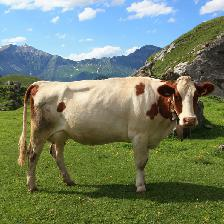
\includegraphics[width=\textwidth]{img/introduction/cow_original.jpg}
        \caption{Original}
    \end{subfigure}
    \hfill
    \begin{subfigure}[b]{0.22\textwidth}
        \centering
        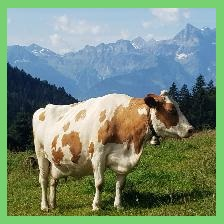
\includegraphics[width=\textwidth]{img/introduction/cow_noise.jpg}
        \caption{Sampling}
    \end{subfigure}
    \hfill
    \begin{subfigure}[b]{0.22\textwidth}
        \centering
        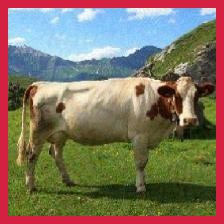
\includegraphics[width=\textwidth]{img/introduction/cow_fgsm.jpg}
        \caption{Adversarial}
    \end{subfigure}
    \hfill
    \begin{subfigure}[b]{0.22\textwidth}
        \centering
        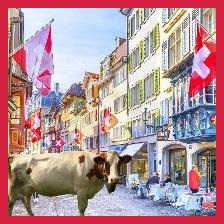
\includegraphics[width=\textwidth]{img/introduction/cow_ood.jpg}
        \caption{Domain}
    \end{subfigure}
       \caption{Illustrative example of three sources of variability
       mentioned. A pre-trained MobileNetV2 
       architecture is shown to be vulnerable to adversarial perturbations 
       as the one represented in (c), and also to domain shifts 
       as the one illustrated in (d), possibly because its inductive bias is influenced
       by the spurious correlation between cows and their natural background.}
       \label{fig:cows}
\end{figure}

This thesis will encompass both phenomena under the same theoretical
framework, and devise a common approach to the measurement of
the distribution shift entailed by both adversarial and domain
variability. Robustness will be characterized from the space of
outcomes of the model, by means of a (posterior) probability 
distribution that will rank models and methods according to the
agreement in their predictions when subject to different noise instantiations.

\subsection{Adversarial setting}

As it was already mentioned, certain perturbations of
original test images, which can be almost imperceptible
to the human eye, can lead to high-confidence
incorrect predictions by deep neural networks, even when their
standard performance metrics are high.
Adversarial examples have been shown to transfer
across architectures and training procedures, and
even across subsets of data,
often yielding the same incorrect prediction in
all of these cases \cite{szegedyIntriguingPropertiesNeural2014}. \\

These intriguing phenomena were initially hypothesized to arise 
from a lack of smoothness over the input space, a property
commonly assumed in other learners, deriving from their
non-linear nature. Nevertheless,
extensive research on the field has ellucidated that the root
cause is instead the linearity of its learning units, which makes them
vulnerable in certain directions of high-dimensional
spaces where small
effects can add up to significally change the outcome
\cite{goodfellowExplainingHarnessingAdversarial2015}. \\

Following this intuition, several attacks have been proposed
to evaluate the robustness of models to adversarial examples by
finding vulnerable directions and adjusting the perturbation to have
the desired misleading effect.  Adversarial examples generated
by these attacks can be used to train robust models via regularization,
pushing generalization to those features present in the worst-case
bounded perturbations and thus selecting models insensitivized
to them. \\

Nevertheless, adversarial learning entails decision boundaries 
that are more complex than the ones derived via standard training
(see Figure \ref{fig:adversarial_complexity}), 
intuitively demanding more data and more complex 
architectures, at the risk of
overfitting to adversarial examples themselves
\cite{schmidtAdversariallyRobustGeneralization2018}. 
These limitations express a fundamental trade-off 
that arises from an intrinsic 
difference between robust and non-robust features
\cite{tsiprasRobustnessMayBe2019, zhangTheoreticallyPrincipledTradeoff2019}. \\

\begin{figure}[h]
    \centering
    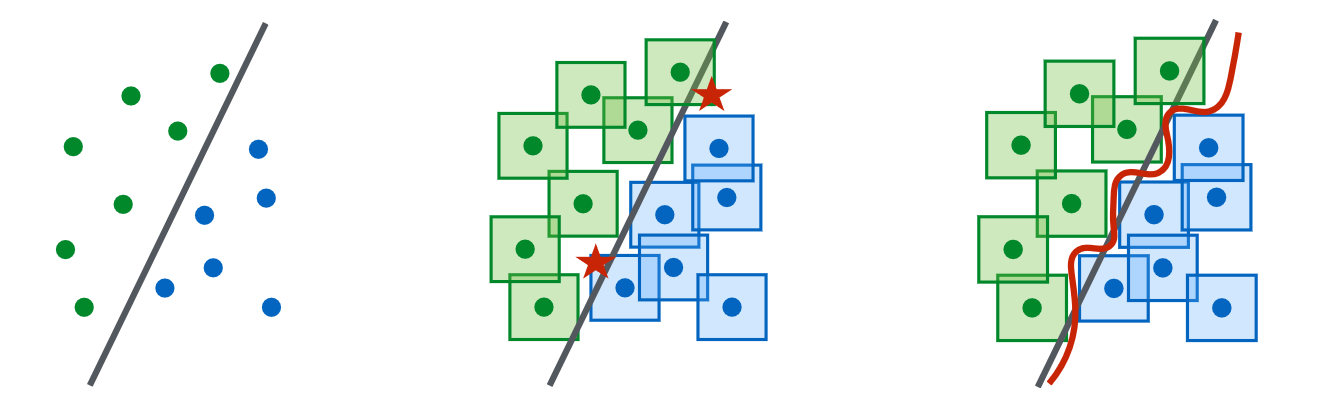
\includegraphics[width=0.7\textwidth]{img/introduction/adversarial_complexity.png}
    \caption{
    A conceptual illustration of standard vs. adversarial 
    decision boundaries. (\textbf{left}) A set of linearly-separable points. 
    (\textbf{middle}) Decision boundary learned via standard training.
    (\textbf{right}) Decision boundary learned via adversarial training.
    Both methods achieve zero training error, but only the robust model
    is able to generalize to $\ell_\infty$ perturbations.
    Source: \cite{madryDeepLearningModels2019}
    }
    \label{fig:adversarial_complexity}
\end{figure}

%\begin{figure}[H]
%    \centering
%    \begin{subfigure}[b]{0.3\textwidth}
%        \centering
%        \includegraphics[width=\textwidth]{img/introduction/adversarial_db_1.jpg}
%    \end{subfigure}
%    \hspace{1cm}
%    \begin{subfigure}[b]{0.3\textwidth}
%        \centering
%        \includegraphics[width=\textwidth]{img/introduction/adversarial_db_2.jpg}
%    \end{subfigure}
%    \caption{(left) Decision boundary learned via standard training. 
%    (right) Decision boundary learned by an adversarial training method, where 
%    the orange dotted line represents the decision boundary in the left figure.
%    Both methods achieve zero training error, but only
%    the robust model is able to generalize to adversarial examples. 
%    Source: \cite{zhangTheoreticallyPrincipledTradeoff2019}}
%    \label{fig:decision_boundaries}
%\end{figure}

Features selected by standard training
are the most predictive towards generalization
to sampling randomness within the same dataset, but they do
not necessarily represent the features implicitly selected 
by humans and are not invariant to a human-based notion 
of similarity. Instead, features selected via adversarial training 
have been shown to represent this
invariance, and thus align much better with 
human perception (see Figure \ref{fig:adversarial_loss})
\cite{ilyasAdversarialExamplesAre2019}. 

\begin{figure}[H]
    \centering
    \begin{subfigure}[b]{0.35\textwidth}
        \centering
        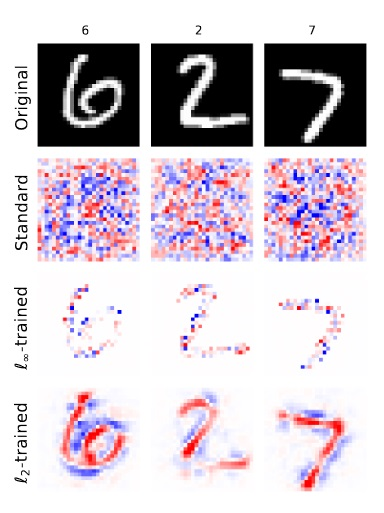
\includegraphics[width=\textwidth]{img/introduction/adversarial_loss_1.jpg}
        \caption{MNIST}
    \end{subfigure}
    \hspace{1cm}
    \begin{subfigure}[b]{0.35\textwidth}
        \centering
        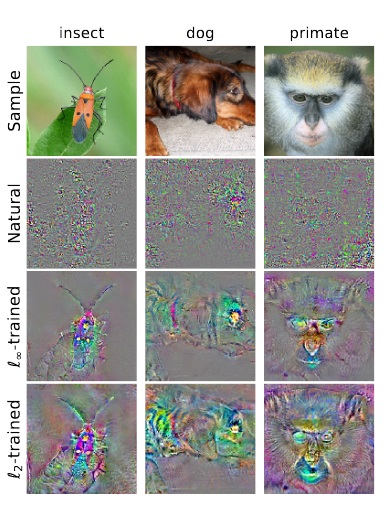
\includegraphics[width=\textwidth]{img/introduction/adversarial_loss_2.jpg}
        \caption{Restricted ImageNet}
    \end{subfigure}
       \caption{Scaled loss gradient with respect to input images.
       Input pixels yielding the most predictive power are aligned 
       with perceptually relavant features for the case of adversarial
       models, while appearing completely random in the case of 
       standard models.
       Source: \cite{tsiprasRobustnessMayBe2019}}
       \label{fig:adversarial_loss}
\end{figure}

Furthermore, adversarial perturbations of robust models have 
been shown to display salient characteristics;
that is, their features are perceived to belong to the
class they are "misclassified" to, as it is illutrateed in 
Figure \ref{fig:salient_characteristics}. 

\begin{figure}[H]
    \centering
    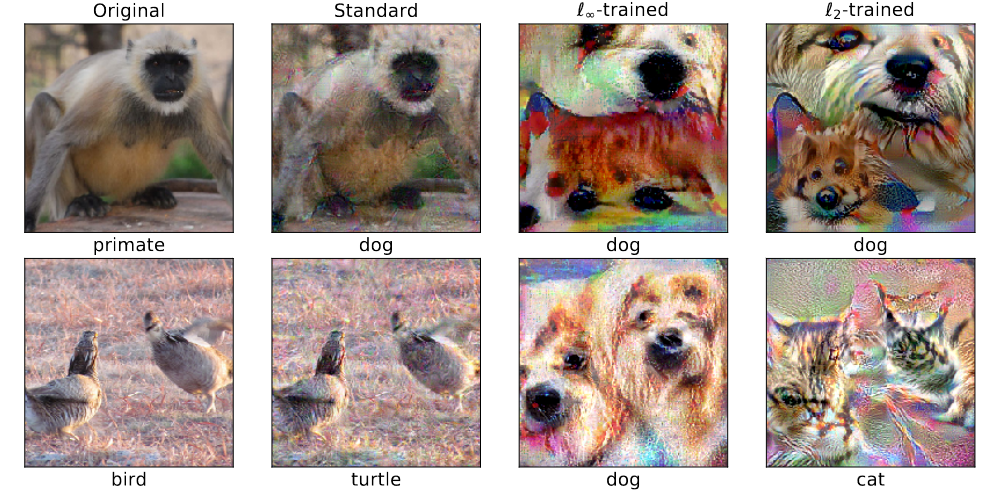
\includegraphics[width=0.5\textwidth]{img/introduction/adversarial_salient.png}
    \caption{Adversarial examples for standard and PGD-trained models.
    Perturbed images produced for robust models 
    effectively capture salient data characteristics and 
    appear similar to examples of a different class. 
    Source: \cite{tsiprasRobustnessMayBe2019}}
    \label{fig:salient_characteristics}
\end{figure}

Overall, these and other findings suggest that robustness in the adversarial setting
is a fundamental property of data rather than models, and
the phenomenon of transferability can be explained in
these terms. Training strategies that are able to navigate the 
robustness-generalization trade-off will be the ones providing 
the best results, provided that the data distribution
is representative of the true underlying features. \\

\subsection{Out-of-distribution setting}\label{sec:intro_ood}

Most learning algorithms work under the fundamental assumption that
a causal relationship exists between input and output spaces and
the target function to learn represents that causality and thus
remains invariant regardless of the available data,
implying that suitable approximations of this 
function can be obtained when data samples are independent 
and identically distributed in the input space
\cite{muandetDomainGeneralizationInvariant2013,quinonero-candelaDatasetShiftMachine2009}. 
Nevertheless, this is not always
the case, as often real-world data does not match the same statistical
patterns as the data used for training, which defines a
distribution shift that leads to poor generalization performance
\cite{zhouDomainGeneralizationSurvey2022,wangGeneralizingUnseenDomains2022,liuOutOfDistributionGeneralizationSurvey2023}. \\

\begin{figure}[H]
    \centering
    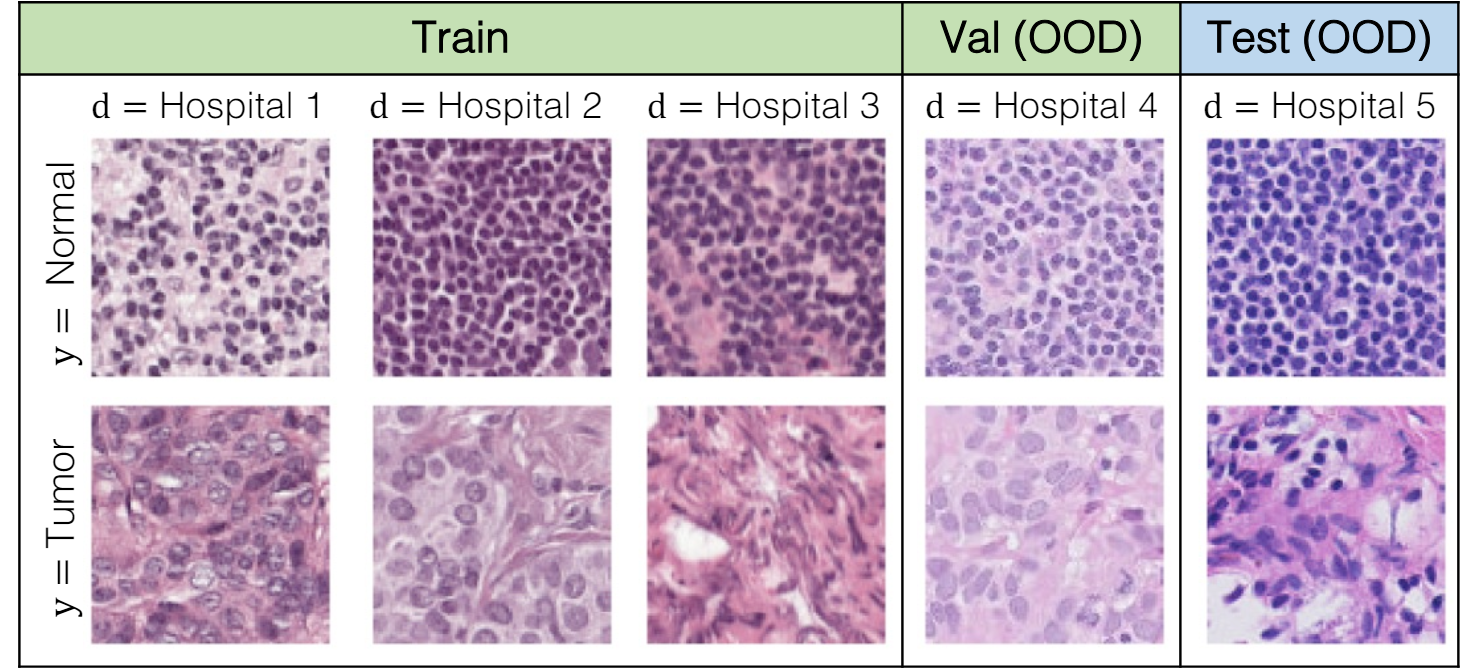
\includegraphics[width=0.6\textwidth]{img/introduction/camelyon17.png}
    \caption{The \texttt{camelyon17} (WILDS) dataset comprises tissue patches from 
    different hospitals. The goal is to accurately predict the presence of 
    tumor tissue in patches taken from hospitals that are not in the 
    training set.
    Source: \cite{kohWILDSBenchmarkIntheWild2021}
    }
    \label{fig:camelyon17}
\end{figure}

A distribution shift can arise for various reasons, namely the 
unfeasibility of collecting diverse enough data, the lack of 
representativity of certain features, the changing or time-dependent
nature of the data and also the implicit bias
induced in the data collection process. This last point
is particularly relevant, as it can serve as a generalization of all
the previous cases and raise epistemological questions
about the learning framework itself. For instance, 
Figure \ref{fig:dataset_bias} refers to a cross-generalization analysis in which popular
machine learning datasets were shown to be biased towards
specific representation of features. Considering the fact that all
data is sampled from the same source (i.e. internet), 
numerous human-induced biases are shown to determine the 
nature of representations, the most significant of all being 
negative bias, which arises when the negative subset\footnote{
    When certain observations in a dataset are labelled as belonging 
    to a specific class, the remaining observations are implicitly
    assigned to not belong to that class, and therefore define a
    negative set in the model feature space.
}
of the dataset is not representative of the input subspace 
excluding that  particular class and results in a model that performs 
significantly worse in other datasets, even when trained with 
the same observations of that class.\\

Several approaches can be taken to address this issue, depending
on the nature of the distribution shift and the access to its
causal structure (see Figure 3 and Table 2 in 
\cite{wangGeneralizingUnseenDomains2022}).
Nevertheless, the common goal is to push the model towards
domain-invariant representations that foster robustness in the
face of distribution shifts, sometimes relaxing the causality condition
to an assumption of invariance or stability of the distribution in the output space
\cite{wangGeneralizingUnseenDomains2022,liuOutOfDistributionGeneralizationSurvey2023}. \\

\begin{figure}[H]
    \centering
    \begin{subfigure}[b]{0.35\textwidth}
        \centering
        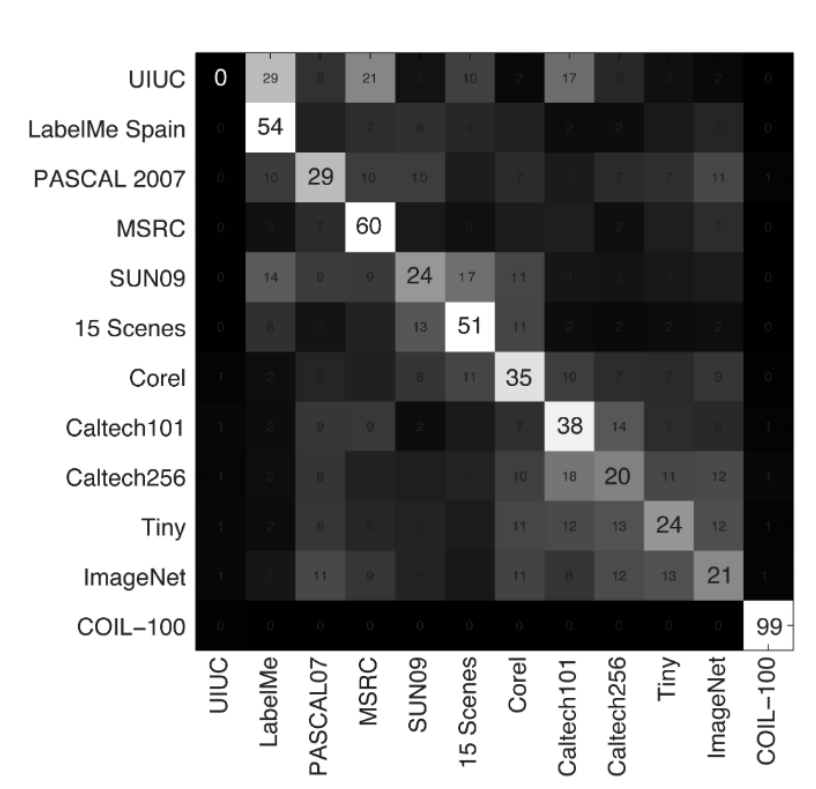
\includegraphics[width=\textwidth]{img/introduction/dataset_bias_confusion.png}
    \end{subfigure}
    \hspace{1cm}
    \begin{subfigure}[b]{0.32\textwidth}
        \centering
        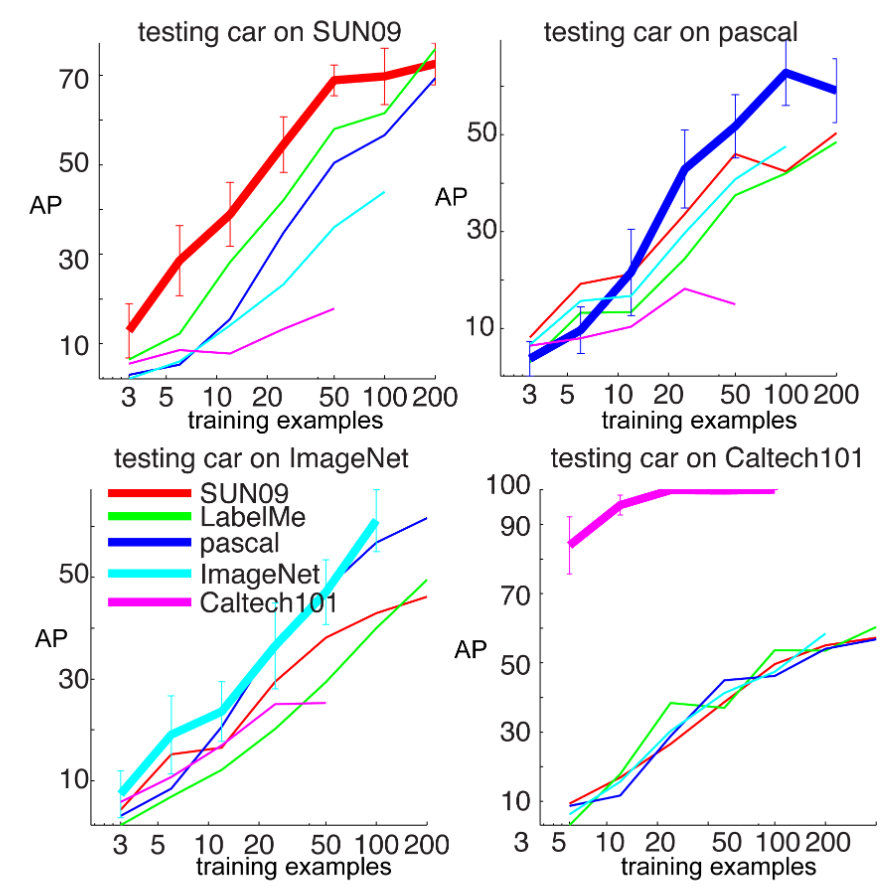
\includegraphics[width=\textwidth]{img/introduction/dataset_bias_cross_generalization.png}
    \end{subfigure}
       \caption{
        \textbf{(left)} Confusion matrix associated with a dataset
        identification task. There is a clearly pronounced diagonal,
        which indicates that each dataset posesses unique traits that
        make it distinguishable from the rest.
        \textbf{(right)} Cross-dataset generalization
        for "car" detection as function of training data. The vertical 
        gap between two curves represents the decrease in performance 
        resulting from training on a different dataset, and horizontal 
        shift corresponds to the increase in amount of data needed 
        to reach the same level of performance.
        Source: \cite{torralbaUnbiasedLookDataset2011}}
       \label{fig:dataset_bias}
\end{figure}

In general, every formulation considers a set of source domains 
encompassing data that is available for the training of the model,
including any validation subsets used for model selection, 
regularization, or other hyperparameter tuning, and a set of target 
domains encompassing unseen data on which model performance will
be evaluated. Within this framework, a straightforward approach
to improving robustness is to directly sample target domains
and adjust feature representations to be invariant 
between both, which is known as domain adaptation. \\

In this work we will focus instead on domain generalization, which 
refers to the case in which sampling from target domains is 
not feasible and feature invariance can be only enforced 
from the source
\cite{blanchardGeneralizingSeveralRelated}. In particular, two strategies will be considered, 
namely domain alignment and data augmentation/generation. \\

On the one hand, domain alignment stems from the output stability condition, and can be 
formulated as a regularization problem that pushes towards the 
minimization of the dissimilarity of feature  representations originated 
from different source environments. The feature space in which the 
alignment is performed (e.g. kernel latent space 
\cite{muandetDomainGeneralizationInvariant2013}, 
adversarial
\cite{peiMultiAdversarialDomainAdaptation}
or model-based
\cite{arjovskyInvariantRiskMinimization2020}) 
and the similarity metric will
determine the the particularities of the method
\cite{shenWassersteinDistanceGuided2018,liangComprehensiveSurveyTestTime2023}.

\begin{figure}[H]
    \centering
    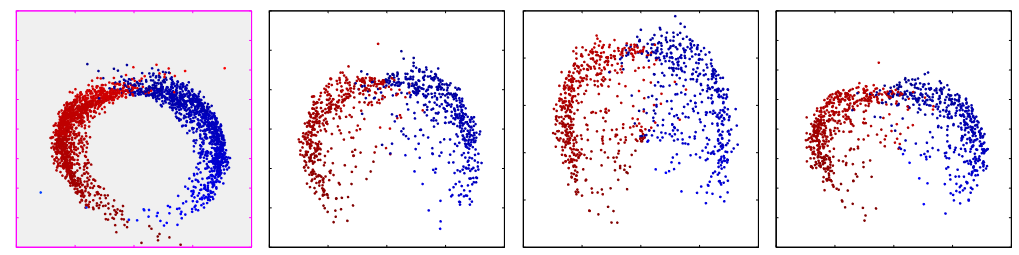
\includegraphics[width=0.67\textwidth]{img/introduction/dica.png}
    \caption{
    Projections of a binary synthetic dataset in the two principal DICA
    dimensions. The shaded box depicts the projection of training 
    data, whereas the unshaded boxes show projections of unseen 
    test datasets. Source: \cite{muandetDomainGeneralizationInvariant2013}
    }
    \label{fig:dica}
\end{figure}

On the other hand, data augmentation/generation strategies 
do not need to assume output stability and instead 
achieve cross-domain generalization by generating new samples that
diversify the original dataset with the hope of capturing 
the underlying causal structure of the problem. Augmented samples
can either be randomizations of original observations (e.g. transformations
such as rescaling or rotations) or new samples filling the distribution
gaps between domains. \\

\begin{figure}[H]
    \centering
    \begin{subfigure}[b]{0.2\textwidth}
        \centering
        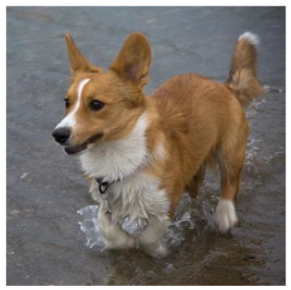
\includegraphics[width=\textwidth]{img/introduction/da_original.png}
        \caption{Original}
    \end{subfigure}
    \hspace{1cm}
    \begin{subfigure}[b]{0.2\textwidth}
        \centering
        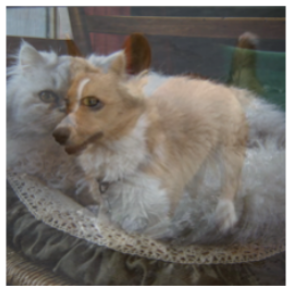
\includegraphics[width=\textwidth]{img/introduction/da_mixup.png}
        \caption{Mixup 
        \cite{zhangMixupEmpiricalRisk2018}
        }
    \end{subfigure}
    \hspace{1cm}
    \begin{subfigure}[b]{0.2\textwidth}
        \centering
        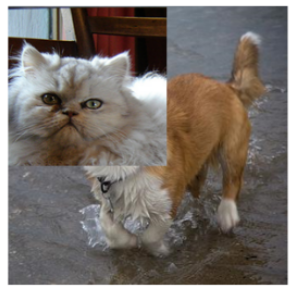
\includegraphics[width=\textwidth]{img/introduction/da_cutmix.png}
        \caption{CutMix
        \cite{yunCutMixRegularizationStrategy2019}
        }
    \end{subfigure}
       \caption{
        Mixup and Cutmix strategies can be used to interpolate
        between different labels and/or domains
        by generating intermediate observations.
        Source: \cite{yunCutMixRegularizationStrategy2019}
        }
       \label{fig:data_augmentation}
\end{figure}

Unlike in the adversarial setting, there is no common way of measuring
the shift in distribution betweeen source domains, and current approaches
are often constrained to specific datasets or training strategies. 
Robustness is instead quantified during (cross-)validation, either by reserving
a subset of each domain, leaving one domain out, or
by directly accessing target domains if they are available, 
which is known as the oracle approach. This last strategy is often
used to provide an upper bound estimate of model robustness, 
as it usually provides over-confident performance estimates
\cite{zhouDomainGeneralizationSurvey2022}.
Numerous benchmark datasets, some of which will be considered in this work, are the current 
standard for robustness assessment even with
the limitations they present
\cite{kohWILDSBenchmarkIntheWild2021}. 
\\

%Despite extensive research on the field and a wide variety
%of strategies envisionated, robustness to distribution shifts 
%continues to pose a fundamental challenge in machine learning. As
%previously mentioned, this difficulty primarily arises from the 
%violation of the sampling uniformity assumption, which renders 
%conventional learning techniques ineffective, and also from the 
%lack of a universal formal characterization of distribution shifts.
%Existing benchmark datasets, some of which will be considered in this work, are the current 
%standard for robustness assessment even with
%the limitations they present. \\

\section{Related work}

In the adversarial front, early work 
\cite{szegedyIntriguingPropertiesNeural2014}
unveiled the nature of the susceptibility of deep learning 
models to adversarial examples and FGSM 
\cite{goodfellowExplainingHarnessingAdversarial2015}
was introduced as an intuitive
approach for model regularization. 
Since then, several gradient-based methods have been
proven to enhance adversarial robustness, such as PGD
\cite{madryDeepLearningModels2019}, C\&W 
\cite{carliniEvaluatingRobustnessNeural2017},
FMN
\cite{pintorFastMinimumnormAdversarial2021} and
many others (see 
\cite{liReviewAdversarialAttack2022} for reference). 
All of them ultimately entail a strategy to find
a vulnerable direction and adjust the perturbation 
(e.g. minimum-norm, maximum-confidence, etc.)
based on the location of the decision boundary, either via soft
constraints (i.e. regularization), boundary attacks or gradient
projections
\cite{baiRecentAdvancesAdversarial2021}. \\

In general, the primary distinction among adversarial attacks lies in
their knowledge of the model's architecture and parameters. In that
sense, white-box and black-box
attacks can be distinguished, where the former have full 
access to the model and the latter only 
to the model's predictions. In black-box settings the loss gradient
is unknown and other strategies such as score-based or
decision-based attacks are used
\cite{liReviewAdversarialAttack2022}. Regarding adversarial training (i.e. defenses), 
robustness can
be achieved by a variety of methods, 
such as ensemble learning,
defensive distillation,
generative adversarial networks
\cite{xiaoGeneratingAdversarialExamples2019, miyatoVirtualAdversarialTraining2018},
diffusion models
\cite{wangBetterDiffusionModels2023,hoDenoisingDiffusionProbabilistic2020}
and adaptive-boundary methods
\cite{cohenCertifiedAdversarialRobustness2019}.
In this project, the Robustbench benchmark attacks 
\cite{croceRobustBenchStandardizedAdversarial2021a}
computed in the \texttt{CIFAR10} dataset will will
be used as a standard for adversarial robustness evaluation. \\

In the domain generalization front, the existing rich taxonomy 
of methods can be classified into three main groups, namely
data manipulation, representation learning 
and alternative learning strategies
\cite{wangGeneralizingUnseenDomains2022,zhouDomainGeneralizationSurvey2022,liuOutOfDistributionGeneralizationSurvey2023}.
Data manipulation strategies refer to augmentation and generation,
as for example randomization or adversarial augmentation
\cite{yaoImprovingOutofDistributionRobustness2022,zhangMixupEmpiricalRisk2018,yunCutMixRegularizationStrategy2019}.
Representation learning strategies are primarily divided 
into domain-invariant methods (e.g. IRM
\cite{arjovskyInvariantRiskMinimization2020} or
kernel-based
\cite{muandetDomainGeneralizationInvariant2013,arjovskyWassersteinGAN2017}) 
and feature disentanglement methods, which encompass causality-inspired
approaches and general multi-component analysis. Other 
learning strategies include meta-learning
\cite{liLearningGeneralizeMetaLearning2018,wangMetaFineTuningNeural2020},
ensemble learning or self-supervised learning. \\

Regarding robustness characterization, a wide range of metrics
have been conceived (see
\cite{guoComprehensiveEvaluationFramework2023} for reference), but
accuracy-based criteria are still the most common. Alternatively, 
some  theoretically-grounded approaches have been proposed, such
as CLEVER \cite{wengEvaluatingRobustnessNeural2018}, ACTS 
\cite{wangGeometricalApproachEvaluate2023}
or
PA
\cite{buhmannPosteriorAgreementModel2022}, 
which is the one we will explore in this work. 
In general, robustness is often reported and compared using 
robustness benchmark datasets. Some of the most relevant
for image classification tasks are 
MNIST (and its multiple variations, such as DiagVib-6
\cite{euligDiagViB6DiagnosticBenchmark2021}),
PACS
\cite{yuPACSDatasetPhysical2022},
VLCS
\cite{khoslaUndoingDamageDataset2012}
or WILDS
\cite{kohWILDSBenchmarkIntheWild2021}.

\section{Objectives}

WRITE AT THE END \\

The main objective of this thesis is thus to assess
the suitability of this framework in the context of deep 
learning model robustness in image classification tasks. 
For that, an operative version of posterior
agreement will be derived, and an efficient implementation of its
computation will be used as a metric to evaluate and select models
based on the robustness of their response to different sources and
levels of variability. The results of this work will be compared
with the current state-of-the-art in robustness evaluation, namely
robustbench
\cite{croceRobustBenchStandardizedAdversarial2021}
and WILDS 
\cite{kohWILDSBenchmarkIntheWild2021}
benckmarks in the adversarial and
out-of-distribution settings, respectively, and an overall
analysis of the use of the metric as an early-stopping 
criterion will be provided.\\


- Lead to the derivative work that will be presented in the thesis.=> benchmarking \\
- Lead to derivative but next level (more useful, current interest...) work => model selection \\
- Lead to non-derivative (i.e. probably unsuccessful) work => model selection beyond robustness \\
- Outline the structure of the thesis in terms of hypothesis. \\
